\documentclass[12pt]{article}
\usepackage{graphicx}
\usepackage{float}

\title{MSCF Finance\\ Homework Set 1}
\author{
Jordan Giebas
}
\date{\today}

\begin{document}
\maketitle

\section{Question 1}

	\subsection{part a}

		\begin{figure}[h]
		\centering
			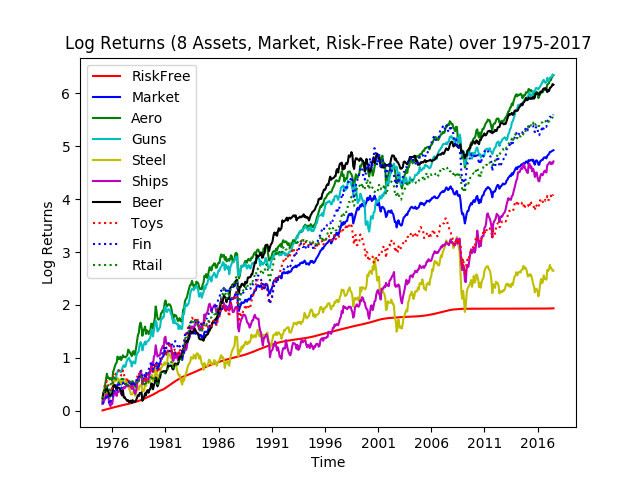
\includegraphics[scale=0.75]{hw1_image1.png}
		\end{figure}

	\subsection{part b}
		
		The market portfolio exhibits characteristics spanning across the entire market, specifically more than these eight different assets. Therefore,
		it is like an average, placing it mainly in the middle rather than primarily above or below any specific asset. The market is constantly reacting to 
		supply and demand, and seeing a drop in one particular asset may simultaneously occur while there is a upward momentum in another (and vice-versa). 
		This being said, the middle is a good fit for it. 
		
	\subsection{part c}
	
		\begin{itemize}
		
			\item October 19, 1987: "Black Monday" (or "Black Tuesday"), this financial crisis began in Hong Kong, went through London, and arrived with shock in the U.S.
					  Although a variety of volatile events were occurring around that time (London closing early due to 'The Great Storm', the U.S. responding to the Iran's
					  silkworm missile attack, and the collapse of OPEC), the popular opinion asserts that the crash was due to 'program traders' (i.e. quants, fantastic). 
					  
			\item Early 2000s recession: This is more widely, and informally, known as the 'dot-come bubble'. Despite the 1997 financial crisis in Asia, and the lesser known
					  problems in the early 1990s in the United States, the market was proliferating in the late 1990s, early 2000s. This was due in large part to the growth of the
					  internet, and the excessive speculation for the 'age of the internet' during that time. 
					  
			\item 2008 Financial Crisis: This is the most recent of the crises, and probably the most widely 'known'. Many claim to understand the causality of the financial crisis 
					  in 2007-2009, attributing the crash mainly to the fraudulent loans underwritten within MBS. Despite this rather mundane point, Gorton offers a refreshing take 
					  on the crisis and the other factors, such as , that eventually led to the crisis felt by so many.
		
		\end{itemize}				
		
\newpage

\section{Question 2}
		
		\subsection{part (a), (b), (c)}
		
			\begin{center}
 			\begin{tabular}{||c|c|c|c||} 
 				\hline
 					Asset & Annual Average Excess Return & Annual Variance & Sharpe Ratio \\
 				\hline\hline
 					Market & 0.08 & 0.024 & 0.452 \\ 
 				\hline
					Aero & 0.114 & 0.051 & 0.461 \\
 				\hline
 					Guns & 0.114 & 0.049 & 0.47 \\
 				\hline
 					Steel & 0.027 & 0.075 & 0.062 \\
 				\hline
 					Ships & 0.075 & 0.067 & 0.251 \\
				 \hline
				  	Beer & 0.11 & 0.031 & 0.568 \\
				 \hline
				  	Toys & 0.061 & 0.056 & 0.216 \\				 
				  \hline
				  	Fin & 0.096 & 0.047 & 0.397 \\
				  \hline
					Rtail & 0.094 & 0.035 & 0.449 \\
				  \hline
					
			\end{tabular}
			\end{center}
			
		\subsection{part (d)}
		
			\begin{figure}[h]
			\centering
				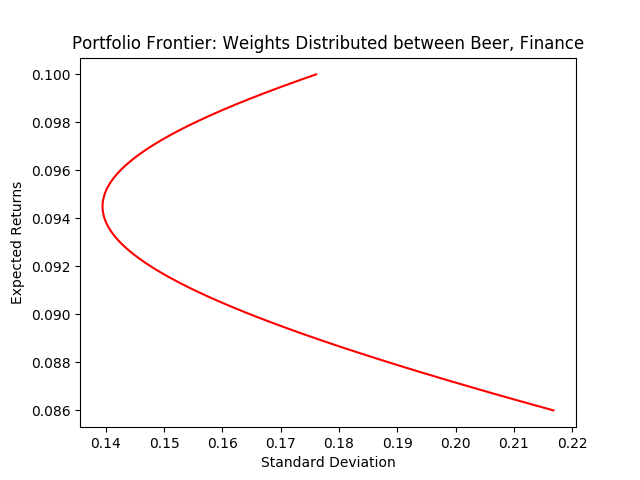
\includegraphics[scale=0.75]{hw1_image2.png}
			\end{figure}
		
		\subsection{part (e)}
		
			To find the tangency portfolio, we determined the weighting that maximizes the Sharpe ratio. \\
			
			\begin{center}
				$SharpeRatio_{max} = 0.608$ \\
				$Portfolio Allocations: [\Delta_{Beer}, \Delta_{Fin}] = [0.65, 0.35]$ \\
			\end{center}
		
\section{Question 3}

	\subsection{part (a)}
	
		Here is a graph of just the efficiency frontier, not the entier mean-variance portfolio. 
	
			\begin{figure}[h]
			\centering
				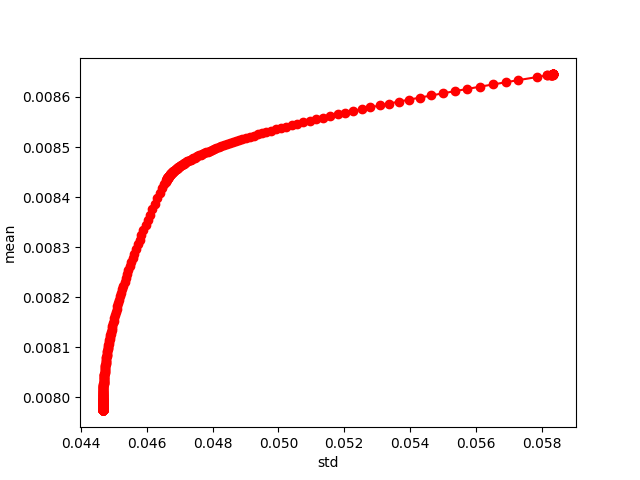
\includegraphics[scale=0.75]{hw1_image3.png}
			\end{figure}
			
			\begin{center}
 			\begin{tabular}{||c|c|c|c||} 
 				\hline
 					Asset & Portfolio Weight \\
 				\hline\hline
					Aero & .02568 \\
 				\hline
 					Guns & 0.97431 \\
 				\hline
 					Steel & 0.0 \\
 				\hline
 					Ships & 0.0 \\
				 \hline
				  	Beer & 0.0 \\
				 \hline
				  	Toys & 0.0 \\				 
				  \hline
				  	Fin & 0.0 \\
				  \hline
					Rtail & 0.0 \\
				  \hline
			\end{tabular}
			\end{center}

This is clearly wrong, but I didn't have enough time to finish it (I realize that's ridiculous since we were given more than 2 weeks, I just didn't realize
how much time the third one would take since I did the first two relatively quickly and left this for the last minute).  I'm using a nonlinear solver in Python
and don't think I set up my constraints the correctly - I'll make sure to better manage my time. \newline

	\subsection{part (b)}
	
		Because of the incorrect answer on Part (a), the Sharpe Ratio I find in Part (b) would be incorrect as well. 

\end{document}




